% ==========================================================================
% Poster TFM — data.lung
% A0 vertical. Estilo editorial: header minimalista, hero de cifras a
% ancho completo, dos columnas amplias, tipografia con jerarquia clara.
% ==========================================================================
\documentclass[25pt, a0paper, portrait, margin=20mm, innermargin=15mm,
               blockverticalspace=14mm, colspace=18mm, subcolspace=10mm]{tikzposter}

\usepackage[utf8]{inputenc}
\usepackage[T1]{fontenc}
\usepackage[spanish,es-tabla]{babel}
\usepackage{lmodern}
\usepackage{graphicx}
\usepackage{booktabs}
\usepackage{xcolor}
\usepackage{amssymb}
\usepackage{tikz}
\usepackage{fontawesome5}
\usetikzlibrary{arrows.meta, positioning, shapes.geometric, fit, calc}

\tikzposterlatexaffectionproofoff

% ================================================================
% Paleta editorial: verde terminal como acento, gris casi negro para
% texto, blancos y grises muy claros para superficies. Nada de bloques
% rellenos de color.
% ================================================================
\definecolor{ink}{HTML}{0B0B0B}
\definecolor{ink2}{HTML}{4A4948}
\definecolor{inkMute}{HTML}{9A9894}
\definecolor{line}{HTML}{D8D6CE}
\definecolor{surface}{HTML}{FFFFFF}
\definecolor{plane}{HTML}{FAF8F2}
\definecolor{verdeTerm}{HTML}{1C8A3F}
\definecolor{verdeOsc}{HTML}{146A2F}
\definecolor{amber}{HTML}{C78A1E}

\definecolorpalette{editorial}{
  \definecolor{colorOne}{named}{verdeTerm}
  \definecolor{colorTwo}{named}{ink}
  \definecolor{colorThree}{named}{plane}
}

\definecolorstyle{editorial}{}{
  \colorlet{backgroundcolor}{white}
  \colorlet{framecolor}{white}
  \colorlet{titlefgcolor}{ink}
  \colorlet{titlebgcolor}{white}
  \colorlet{blocktitlebgcolor}{white}
  \colorlet{blocktitlefgcolor}{ink}
  \colorlet{blockbodybgcolor}{white}
  \colorlet{blockbodyfgcolor}{ink}
  \colorlet{innerblocktitlebgcolor}{white}
  \colorlet{innerblocktitlefgcolor}{ink}
  \colorlet{innerblockbodybgcolor}{plane}
  \colorlet{innerblockbodyfgcolor}{ink}
  \colorlet{notefgcolor}{ink}
  \colorlet{notebgcolor}{plane}
  \colorlet{notefrcolor}{verdeTerm}
}

\usetheme{Empty}
\usecolorstyle{editorial}
\usebackgroundstyle{Plain}
\usetitlestyle{Empty}

% Bloque estilo editorial: sin relleno, solo un filete verde bajo el
% titulo y un poco de aire debajo.
\defineblockstyle{editorial}{
  titlewidthscale=1, bodywidthscale=1,
  titleleft, titleoffsetx=0pt, titleoffsety=0pt,
  bodyoffsetx=0pt, bodyoffsety=0pt,
  bodyverticalshift=8mm, roundedcorners=0, linewidth=0pt,
  titleinnersep=6mm, bodyinnersep=6mm
}{
  % Sin fondo ni borde en el cuerpo
  \draw[color=verdeTerm, line width=2mm]
    ($(blocktitle.south west)+(0,3mm)$) --
    ($(blocktitle.south east)+(-\linewidth+30mm,3mm)$);
}
\useblockstyle{editorial}

% Titulos de bloque: kicker mono verde + titulo serif grande
\newcommand{\kicker}[1]{{\ttfamily\fontsize{22pt}{22pt}\selectfont\color{verdeTerm}\textbf{#1}}}
\newcommand{\btitle}[2]{%
  \kicker{#1}\\[4mm]%
  {\bfseries\fontsize{42pt}{46pt}\selectfont #2}}

% Numero grande estilo dashboard
\newcommand{\bignum}[3]{%
  \begin{tikzpicture}
    \node[anchor=north west, inner sep=0pt] (n) at (0,0) {%
      {\fontsize{110pt}{110pt}\selectfont\bfseries\color{ink}#1}%
    };
    \node[anchor=north west, below=2mm of n.south west, text width=140mm,
          font=\ttfamily\fontsize{18pt}{22pt}\selectfont, text=inkMute]
         {#2\\\vspace{1mm}{\normalfont\color{ink2}\fontsize{16pt}{18pt}\selectfont #3}};
  \end{tikzpicture}
}

\renewcommand{\baselinestretch}{1.15}

\begin{document}

% ==========================================================================
% CABECERA
% Franja superior blanca con: mark data.lung a la izquierda, chip UAX a
% la derecha, y el titulo grande a continuacion. Filete verde inferior.
% ==========================================================================
% Kicker superior + marca
\node[anchor=north west, inner sep=0pt] at (-\paperwidth/2+40mm, \paperheight/2-25mm) {
  \begin{minipage}{0.9\paperwidth}
    % Barra superior de metadatos
    {\ttfamily\fontsize{22pt}{22pt}\selectfont\color{verdeTerm}\textbf{\textgreater\ }}%
    {\ttfamily\fontsize{22pt}{22pt}\selectfont\color{ink2}%
     TRABAJO DE FIN DE MÁSTER\ \ \textbullet\ \ MÁSTER EN BIOINFORMÁTICA%
     \ \ \textbullet\ \ UNIVERSIDAD ALFONSO X EL SABIO\ \ \textbullet\ \ MADRID 2026}\\[10mm]

    % Marca data.lung gigante
    {\fontfamily{lmtt}\selectfont\fontsize{200pt}{200pt}\selectfont%
     \color{ink}data\textcolor{verdeTerm}{.}lung}\\[6mm]

    % Tagline
    {\itshape\fontsize{40pt}{46pt}\selectfont\color{ink2}%
     Del dataset a una firma génica replicable.}\\[16mm]

    % Titulo del trabajo (serif, mucho aire)
    {\bfseries\fontsize{54pt}{62pt}\selectfont\color{ink}%
     Framework transcriptómico basado en la integración de modelos\\
     de lenguaje y aprendizaje automático para la identificación\\
     de biomarcadores en cáncer de pulmón}\\[14mm]

    % Autor + tutor en una linea con separadores
    {\fontsize{26pt}{28pt}\selectfont\color{ink}\bfseries%
     Daniel Tapia Díez}%
    \hspace{6mm}%
    {\ttfamily\fontsize{22pt}{24pt}\selectfont\color{inkMute}\textbullet}%
    \hspace{6mm}%
    {\fontsize{22pt}{24pt}\selectfont\color{ink2}%
     Tutor: Leonardo Dulcetti}%
    \hspace{6mm}%
    {\ttfamily\fontsize{22pt}{24pt}\selectfont\color{inkMute}\textbullet}%
    \hspace{6mm}%
    {\fontsize{22pt}{24pt}\selectfont\color{ink2}%
     14 de agosto de 2026}
  \end{minipage}
};

% Filete verde separador de cabecera
\draw[color=verdeTerm, line width=3mm]
  (-\paperwidth/2+40mm, \paperheight/2-500mm) --
  (\paperwidth/2-40mm, \paperheight/2-500mm);

% ==========================================================================
% HERO DE CIFRAS a ancho completo bajo el filete
% ==========================================================================
\node[anchor=north west, inner sep=0pt] at (-\paperwidth/2+40mm, \paperheight/2-520mm) {
  \begin{minipage}{0.9\paperwidth}
    {\ttfamily\fontsize{22pt}{22pt}\selectfont\color{verdeTerm}\textbf{> }%
     CIFRAS CLAVE DEL FRAMEWORK}\\[10mm]

    \begin{tabular}{@{\hspace{0mm}}p{200mm}p{200mm}p{200mm}p{200mm}@{}}
      \bignum{1174}{GENES}{replicados en 3 cohortes independientes} &
      \bignum{20}{PANEL MÍNIMO}{con AUC 0,966 en LODO} &
      \bignum{18/20}{MARCADORES IHC}{recuperados sin declararlos} &
      \bignum{0,968}{AUC LODO}{subtipo ADC vs escamoso} \\
    \end{tabular}
  \end{minipage}
};

% Filete gris fino separador del hero
\draw[color=line, line width=1mm]
  (-\paperwidth/2+40mm, \paperheight/2-750mm) --
  (\paperwidth/2-40mm, \paperheight/2-750mm);

% ==========================================================================
% Cuerpo: dos columnas amplias
% ==========================================================================
\begin{columns}

% -------- COLUMNA IZQUIERDA --------------------------------------------
\column{0.5}

\block{\btitle{I}{Contexto \& objetivo}}{
  El cáncer de pulmón es la \textbf{primera causa de mortalidad
  oncológica} en el mundo (2,48 millones de casos nuevos en 2022;
  supervivencia a 5 años \mbox{$<20$\,\%}).

  \vspace{4mm}
  La distinción entre \textbf{adenocarcinoma} (ADC) y \textbf{carcinoma
  escamoso} (SQC) condiciona el tratamiento: pemetrexed y bevacizumab
  están contraindicados en escamoso. Las bases de datos públicas (NCBI
  GEO) reúnen cientos de estudios pero su integración se ve frenada por
  la heterogeneidad de plataformas y por metadatos clínicos redactados
  en texto libre.

  \vspace{6mm}
  \begin{tikzpicture}
    \draw[color=verdeTerm, line width=1mm] (0,0) -- (25mm,0);
  \end{tikzpicture}\\[3mm]
  {\itshape\fontsize{34pt}{40pt}\selectfont\color{ink}%
   Un framework reproducible que \emph{automatiza} la integración
   multi-cohorte usando un modelo de lenguaje para curar metadatos,
   y \emph{valida externamente} las firmas génicas identificadas.}
}

\block{\btitle{II}{Pipeline}}{
  \centering
  \begin{tikzpicture}[node distance=8mm and 8mm, font=\fontsize{20pt}{22pt}\selectfont]
    \tikzset{
      p/.style={rectangle, draw=line, line width=0.4mm, fill=surface,
                minimum width=54mm, minimum height=18mm, align=center,
                inner sep=2mm},
      entrada/.style={p, fill=plane, draw=verdeTerm, line width=0.6mm},
      salida/.style={p, fill=plane, draw=amber, line width=0.6mm},
      f/.style={-{Latex[length=5mm]}, thick, color=inkMute}
    }
    \node[entrada] (geo) {NCBI GEO};
    \node[p, right=of geo] (des) {\textbf{1} Descarga};
    \node[p, right=of des] (nor) {\textbf{2} Normaliza};
    \node[p, below=of des] (llm) {\textbf{3} LLM curación};
    \node[p, right=of llm] (cri) {\textbf{4} Criterios\\de inclusión};
    \node[p, below=of llm] (dif) {\textbf{5} Welch + FDR};
    \node[p, right=of dif] (ml)  {\textbf{6} LASSO L1\\RF · SVM};
    \node[p, below=of dif] (lod) {\textbf{7} LODO};
    \node[p, right=of lod] (con) {\textbf{8} Consenso\\multi-cohorte};
    \node[salida, below=of lod] (fir) {\textbf{9} Firma\\1174 genes};
    \node[salida, right=of fir] (pan) {\textbf{9} Panel\\mínimo 20};
    \draw[f] (geo) -- (des);
    \draw[f] (des) -- (nor);
    \draw[f] (nor.south) |- (llm.east);
    \draw[f] (llm) -- (cri);
    \draw[f] (cri.south) |- (dif.east);
    \draw[f] (dif) -- (ml);
    \draw[f] (ml.south) |- (lod.east);
    \draw[f] (lod) -- (con);
    \draw[f] (con.south) |- (fir.east);
    \draw[f] (fir) -- (pan);
  \end{tikzpicture}
  \\[6mm]
  \raggedright
  \textbf{Consenso multi-cohorte}: un gen entra en la firma sólo si
  mantiene el mismo signo y $|d|>0{,}5$ (Cohen) en las 3 cohortes
  simultáneamente. \textbf{Validación externa Leave-One-Dataset-Out
  (LODO)} sobre cohortes evaluables.
}

\block{\btitle{III}{Rendimiento en validación externa}}{
  \centering
  \fontsize{22pt}{28pt}\selectfont
  \begin{tabular}{@{}l@{\hspace{16mm}}rrrr@{}}
    \toprule
    \bfseries Tarea & \bfseries AUC & \bfseries Bal.\,acc. & \bfseries Sens. & \bfseries Espec. \\
    \midrule
    Tumor \emph{vs.} sano             & \textbf{0,925} & 0,772 & 0,983 & 0,561 \\
    Subtipo ADC \emph{vs.} SQC        & \textbf{0,968} & 0,940 & 0,924 & 0,957 \\
    \midrule
    \emph{Baseline mayoritario}       & --    & 0,609 & --    & --    \\
    \bottomrule
  \end{tabular}
  \\[5mm]
  \raggedright\normalsize\color{ink2}
  \fontsize{22pt}{28pt}\selectfont
  8 cohortes evaluables para tumor \emph{vs.} sano; 3 cohortes GPL570
  independientes ($n=388$) para subtipo. La brecha AUC / bal.\,acc. en
  la primera tarea proviene del desbalance de entrenamiento (938 tumores
  vs 219 controles), corregible con recalibración por cohorte.
}

% -------- COLUMNA DERECHA --------------------------------------------
\column{0.5}

\block{\btitle{IV}{Validación externa contra IHC clínica}}{
  \fontsize{22pt}{28pt}\selectfont
  De los 20 marcadores diagnósticos del panel IHC de la OMS (2015), el
  framework recupera \textbf{18 sin declararlos}:

  \vspace{5mm}
  \begin{tabular}{@{}p{55mm}p{265mm}c@{}}
    \toprule
    \bfseries Linaje & \bfseries Marcadores recuperados & \bfseries Cobertura \\
    \midrule
    Escamoso &
    KRT5, KRT6A, KRT6B, KRT13, KRT14, TP63, DSG3, DSC3, SOX2, PKP1,
    CALML3, S100A2 & \textbf{12/12} \\[3mm]
    Adenocarcinoma &
    NAPSA, NKX2-1, SFTPB, MUC1, SLC34A2, CEACAM6
    \color{inkMute}\emph{(no recuperados: SFTPA1, SFTPC)} & \textbf{6/8} \\
    \bottomrule
  \end{tabular}

  \vspace{6mm}
  {\itshape La firma, seleccionada por criterio estadístico puro,
  coincide con el panel diagnóstico que ya usa la clínica.}
}

\block{\btitle{V}{Panel mínimo $\approx$ firma completa}}{
  \begin{minipage}[t]{0.55\linewidth}
    \vspace{3mm}
    \fontsize{22pt}{28pt}\selectfont
    Con \textbf{20 genes} la AUC media LODO es \textbf{0,966}; con la
    firma completa de 1174 genes es 0,970. La pérdida es menor de 0,01.

    \vspace{5mm}
    El panel es \textbf{clínicamente manejable}: mide sencillamente por
    PCR cuantitativa multiplex o por NanoString nCounter.
  \end{minipage}\hfill
  \begin{minipage}[t]{0.42\linewidth}
    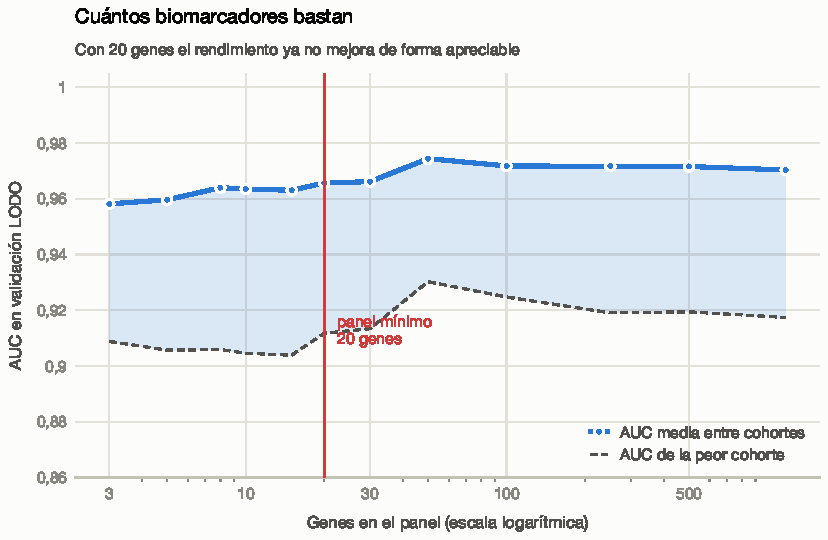
\includegraphics[width=\linewidth]{fig_panel_minimo.pdf}
  \end{minipage}
}

\block{\btitle{VI}{Interpretación biológica: dos ejes reales}}{
  \fontsize{22pt}{28pt}\selectfont
  \textbf{Eje 1 --- Pérdida de arquitectura alvéolo-capilar normal.}
  Correlación media $\rho=-0{,}626$ entre score del clasificador y
  contenido residual de pulmón sano dentro de los tumores; en
  \textbf{GSE31210} ($n=226$) alcanza $\rho=-0{,}858$ con
  $p=1{,}1\cdot 10^{-66}$.

  \vspace{4mm}
  \textbf{Eje 2 --- Actividad proliferativa aumentada.}
  Panel canónico: MKI67, TOP2A, CCNB1, BIRC5, AURKA.

  \vspace{5mm}
  {\itshape Señal biológica reproducible, no artefacto de composición.
  La firma captura la transición del pulmón sano a un tejido menos
  diferenciado y más proliferativo --- la histología del NSCLC.}
}

\block{\btitle{VII}{Conclusiones}}{
  \fontsize{22pt}{30pt}\selectfont
  \begin{itemize}\setlength{\itemsep}{4mm}
    \item Un LLM contemporáneo cura los metadatos de GEO con tasa media
    del \textbf{85,9\,\%}, habilitando la integración multi-cohorte.
    \item El consenso multi-cohorte produce una firma \textbf{robusta}
    (AUC 0,968 LODO en 3 cohortes independientes).
    \item Un panel de \textbf{20 genes} aproxima el rendimiento de la
    firma completa (AUC 0,966 vs 0,970).
    \item La firma \textbf{recupera 18/20 marcadores IHC clínicos}
    sin haberlos declarado, coincidiendo con el panel diagnóstico OMS.
    \item El framework es \textbf{reproducible extremo a extremo}, con
    interfaz web y asistente conversacional integrados.
  \end{itemize}
}

\end{columns}

% ==========================================================================
% Pie: filete + linea de metadatos discreta
% ==========================================================================
\draw[color=line, line width=1mm]
  (-\paperwidth/2+40mm, -\paperheight/2+90mm) --
  (\paperwidth/2-40mm, -\paperheight/2+90mm);

\node[anchor=south, inner sep=0pt] at (0, -\paperheight/2+50mm) {
  \begin{minipage}{0.9\paperwidth}
    \centering\ttfamily\fontsize{20pt}{22pt}\selectfont\color{ink2}%
    {\color{verdeTerm}\textbf{> }}CÓDIGO Y MEMORIA:\ \
    github.com/danitapiadiez-gif/TFM-Bioinformatica
    \hspace{15mm}\textbullet\hspace{15mm}
    INTERFAZ:\ \ streamlit run agentes/paso12\_web\_chatbot.py
    \hspace{15mm}\textbullet\hspace{15mm}
    LICENCIA MIT
  \end{minipage}
};

\end{document}
